\def\year{2015}
%File: formatting-instruction.tex
\documentclass[letterpaper]{article}
\usepackage{float}
\usepackage{aaai}
\usepackage{times}
\usepackage{helvet}
\usepackage{courier}
\usepackage{graphicx}
\usepackage{subfigure}
\usepackage{amsmath}
\usepackage{cases}
\usepackage{multirow}
\usepackage{array}
\usepackage{amssymb}
\usepackage{color}
\usepackage{algorithm}
\usepackage{algorithmic}
\frenchspacing
\setlength{\pdfpagewidth}{8.5in}
\setlength{\pdfpageheight}{11in}
\pdfinfo{
/Title (LSH-Draft)
/Author (Put All Your Authors Here, Separated by Commas)}
\setcounter{secnumdepth}{0}  
 \begin{document}
% The file aaai.sty is the style file for AAAI Press 
% proceedings, working notes, and technical reports.
%

% edit & comments
\newcommand{\xhedit}[1]{{\color{blue} #1}}
\newcommand{\xhcomment}[1]{\xhedit{[XH: #1]}}

% math symbols
% influence strength
\newcommand{\ISM}{A}
\newcommand{\IS}{\alpha}

% popularity of story (diffusion speed or activation probability)
\newcommand{\DS}{P}

% number of Activation node
\newcommand{\NActNodes}{N}


\title{Learning networks of heterogeneous information popularity}
\author{AAAI Press\\
Association for the Advancement of Artificial Intelligence\\
2275 East Bayshore Road, Suite 160\\
Palo Alto, California 94303\\
}
\maketitle
\begin{abstract}
\quad With the increasing popularity of the social networks and information-sharing platforms, many researches about network inference problem have been proposed to deal with such cases when we can only observe the activation time of nodes but the structure of networks are unavailable. In empirical analysis, we observe the fact that previous algorithms have long ignored the heterogeneity of diffusion speed in different life stages, which can result in unsatisfactory Network Inference results. We aim to improve the performance of inference by imposing some transplantable modification on existing method in which the extracted diffusion speed information is well used. But as the estimation of diffusion speed requires parent relationship that is seldom available, we propose a surrogate approach and prove its validity by calculating their correlation. An optimization method of averaging the life span to reduct noise in single cascade is introduced. Experiments on both synthetic dataset and real world dataset show significant improvement on inference accuracy when applying our method.

\end{abstract}
%&&&&&&&&&&&&&&&&&&&&&&&&&&&&&&&&&&
\section{Introduction}

\quad Understanding the processes and dynamics of \emph{information diffusion} through networks plays a fundamental role in a variety of domains, such as evaluating the effects of networks in marketing~\cite{domingos:2001,kempe:2003,leskovec:2007a}, monitoring the spread of news, opinions, and scientific ideas via citation networks~\cite{adar:2004,gruhl:2004,leskovec:2005}, and detecting the spread of erroneous information~\cite{dong:2009}.

In practical applications, the underlying diffusion network (e.g. networks on who influenced whom) is often hidden. Therefore, many interesting models have been developed to automatically infer diffusion networks from cascade observations, i.e., timestamps when users post a blog on certain topics or purchase products~\cite{gomez-rodriguez:leskovec:krause:inferring,gomez-rodriguez:balduzzi:schoelkopf:uncovering,yang:zha:mutualExciting,zhou:zha:song:mutualExciting,Wang:Hu:Philip:Li:multiAspect,Daneshmand:Gomez:Song:recovery14,Du:Song:Song:Alex:HeterogeneousInf,Du:Song:Woo:Zha:topicCascade}. 


To be more specific, the diffusion network is usually modeled as a matrix $ISA=\{\IS_{u,v}\}$, where $\IS_{u,v}$ is a parameter as the strength of influence user $u$ has on $v$. Depending on the diffusion model, $\IS_{u,v}$ can stand for the parameter of the delay distribution for information to propagate from $u$ to $v$ or the probability that $v$ publish a related post given that $u$ has published a post previously. The \emph{Network Inference} problem focuses on discovering the all parameters $\IS_{u,v}$ from the observed cascades. 



Most previous work on network inference assume that the strength of influence $\IS_{u,v}$ between $u$ and $v$ remains the same during the whole life of the diffusion processes. We can easily see that this assumption is unrealistic. Consider the propagation of a story in microblog as an example. It is more likely for a user to be influenced by friends to talk about the story when it is popular due to its freshness in the beginning of the propagation. On the contrary, when the story becomes stale and less popular towards the end of its life, it is less likely that one can influence her friends to have interest in it. 


Ignoring the heterogeneity of influence strength in different stages can lead to unsatisfactory solution of the Network Inference problem. Assume that we observe user $v$ posts the same contents immediately after $u$. Existing Network Inference algorithm will treat it as a strong evidence that user $u$ has strong influence on $v$. However, it is also possible that $v$ reposes fast simply because the story is very popular and any of her friends' post will lead to similar rapid response. On the other hand, if the above scenario occurs when the story is not no longer popular, $v$'s rapid response to $u$'s post can be safely treated as strong evidence that $u$ is very influential on $v$. The confusion between strong influence between friends and the popularity of the story leads to the failure in this scenario.  


In this work, we incorporate the heterogeneity of influence strength in different life stage of diffusion process to improve the accuracy of network inference. We design a heuristic referred to as the \emph{Life Stage Heuristics} (LSH) that can be easily applied to any existing network inference algorithm. In our LSH, we model the strength of influence as a function of the diffusion life stage, namely $\IS_{u,v}(t)$ instead of a constant $\IS_{u,v}$ in previous network inference algorithms. We decouple the $\IS_{u,v}(t)$ as a multiplication of two component, a time varying part $\DS(t)$ modeling the popularity of information and a constant part $\IS_{u,v}$ modeling the strength of influence between pairs of individuals. Our formulation decomposes the true strength of influence from the confounding factor of popularity of the information. Moreover, the simplicity of the multiplicative form makes our heuristic easily applicable to any existing network inference algorithms to improve inference accuracy without changes in implementation nor increment in running time.   


The rest of the paper is organized as follows. We first provide empirical evidence on the heterogeneity of influence strength and then provide a method to approximately estimate the popularity in different stages. We then show how our LSH can be applied to three sate-of-art network inference algorithms to improve the inference accuracy. We carry out extensive experiments on both synthetic and real world datasets to test the performance of our algorithms. Finally, we discuss related work and conclude the paper.  

%&&&&&&&&&&&&&&&&&&&&&&&&&&&&&&&&&&
\section{Empirical analysis}
\quad In this section, we carry out empirical analysis on two real world cascades datasets to show that the assumption of constant influence strength does not hold. We then provide a method to estimate the popularity of the information under propagation empirically from the observed cascades. 

\subsection{Existence of influence strength heterogeneity}
\quad In many network inference models, the influence strength parameter $\alpha_{u,v}$ models the speed of diffusion, namely the time it takes for the information to propagation from user $u$ to $v$.  We empirically estimate the average diffusion speed as the inverse of delay time in two real world cascade datsets, Sina microblog and US Patent to show the heterogeneity of influence strength. \xhcomment{Sina dataset contains the hyper-links such as user $u$ reposts one of $v$'s microblog with delay $t_u-t_v$. Patent dataset contains citation links between patent products.}

The estimation process is as follows: we first normalize the span of each cascade to $[0,1]$ and split the interval into ten bins. We treat each bin as one stage of the diffusion process. We estimate the average diffusion speed in each bin as the inverse of delay time $\frac{1}{\Delta_t}$ using the available explicit following information in the datasets. \xhcomment{What is the unit of y-axis? Is it the diffusion speed after normalization? Ans: I think the inverse of diffusion speed is normalized but diffusion speed isn't. As the unit of y-axis contains normalization value, I'm confused about how to express the unit $\sim\sim$} The results on two cascades from each dataset is shown in Figure \ref{fig:PatentHetero}. 
\begin{figure}[h]
\subfigure[Cascades of Sina Microblog dataset]{\centerline{
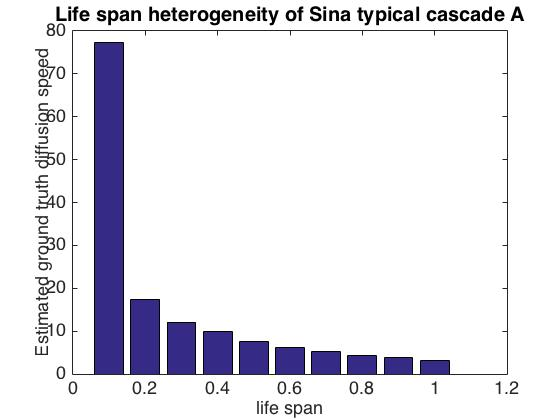
\includegraphics[width=0.55\linewidth]{figures/SinaA.jpg}
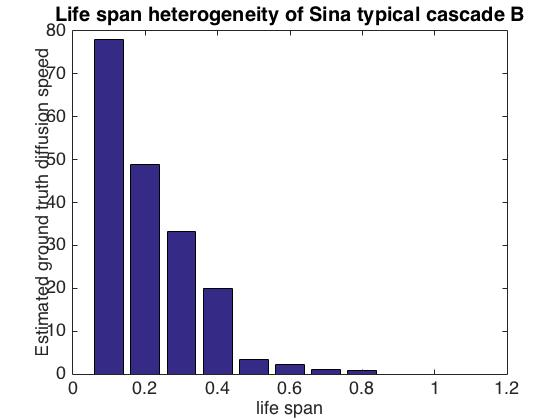
\includegraphics[width=0.55\linewidth]{figures/SinaB.jpg}}}
\subfigure[Cascades of U.S. Patent dataset]{\centerline{
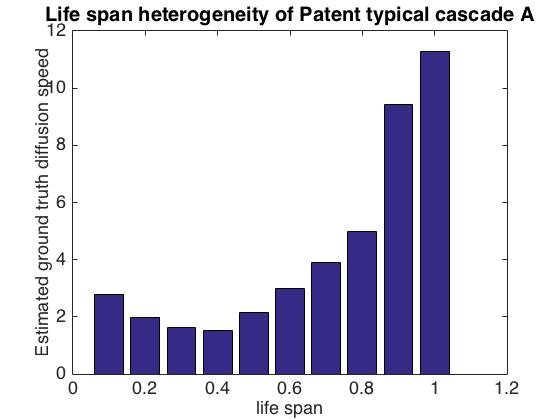
\includegraphics[width=0.55\linewidth]{figures/PatentA.jpg}
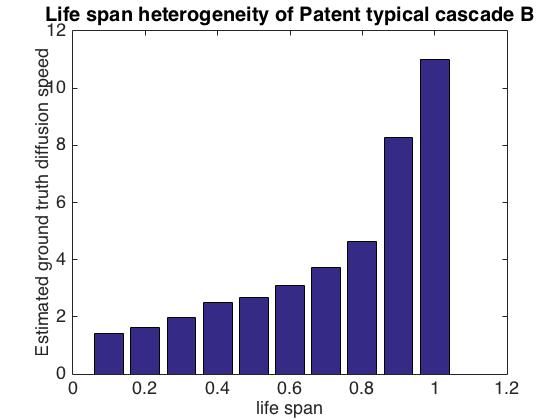
\includegraphics[width=0.55\linewidth]{figures/PatentB.jpg}}}
\caption{The diffusion speed in different stages of diffusion process in two real world datasets. \xhcomment{Could we provide name for each cascade? link the story in microblog and the porduction in patent.  Ans: I'm afraid there is no record in Sina dataset indicating the content of micro-blog; raw data of Patent contains the class of product, such as planting, Jewelry, Bridges, but there can be several different patent classes in a cascade, as one may cite to some patent products in other fields.}}\label{fig:PatentHetero}
\end{figure}

The results clearly demonstrate the deviation from the assumption of constant diffusion speed. Another interesting observation is that the how the diffusion speed depends on the diffusion stages varies dramatically over different cascades and datasets. For the microblog datasets, usually the diffusion speed decrease when the story under propagation becomes stale and less interesting as time elapses. On the contrary, in the patent datsets, newly invented product gradually gains popularity leading to increment in the diffusion speed. 

%It implies that assuming particular functional form of the popularity for all cascades may lead to inaccurate estimation. As a result, we propose to represent the cascade popularity $\DS(t)$ as a piece-wise constant function. Assume we split the normalized span of the cascade into $k$ bins with $t_0=0 < t_1 < \ldots < t_K = 1$. We have $\DS(t) = \DS_i$ if $t\in[t_{i-1}, t_i]$.

%We make an interesting analysis of message's diffusion speed on 2 real world datasets: Sina microblog and U.S. patent. We normalize the activation times with Min-Max method and divide the time length of cascade into several periods.
%As diffusion speed is unmeasurable, we compute the $\frac{1}{\overline{\Delta t}}$ in each life span that is proportion to the ground truth diffusion speed. As in Figure \ref{fig:PatentHetero}, the maximum of $\frac{1}{\overline{\Delta t}}$ reaches 80 in Sina and about 12 in Patent dataset, while the minimum approaches 0. There is distinct difference of diffusion speed in different life span. However, former algorithms have not taken this into consideration. They assume that the coefficient of $\Delta t$'s distribution which controls diffusion speed does not change with time. We believe the life span heterogeneity is a key point to re-understand network inference problem.

%==========================
\subsection{Approximation popularity with number of activation}
\quad Direct estimation of average diffusion speed requires the diffusion pathway which is usually not available in real world datasets. It is even harder to estimate the average activation probability from observed cascades. As a result, we have to seek approximation for the true popularity for different stages in the diffusion process. In the work, we find the total number of activated nodes in each stage of the diffusion process as a good surrogate for the average diffusion speed or the activation probability as a measure for the popularity level. 

Let $I^c(t)$ be the number of activated nodes in cascades $c$ till time $t$. We approximate the popularity level with the following formula:
$$
\DS^c(t) = (I^c(t+\frac{L}{2}) - I^c(t-\frac{L}{2})) / I^c(1).
$$
That is to say, the estimated popularity level at time $t$ is ratio of nodes activated in the windows of length $L$, $[t-\frac{L}{2}, t+\frac{L}{2}]$. 

We carry out experiments to show that the proposed surrogate popularity level is a valid approximation. \xhcomment{We sort all cascades descendingly by activation number and select the top 80 cascades in Patent dataset and top 50 cascades in Sina dataset}. For each cascade, we first normalize the time span to $[0,1]$ and split it into $K$ bins\xhcomment{(we use $k=10$ in this part)}. The true popularity level is assumed to be constant as the average diffusion speed estimated from the particular cascade. We compare the true popularity level and the surrogate popularity at each activation time $t_a$ by computing the Pearson correlation for each cascade. The distribution on the correlation coefficient on the two datasets are shown in Table \ref{tab:Corre}. More than 60\% cascades and 80\% cascades in Patent and Sina microblog dataset respective have correlation coefficient $r>0.6$ with the true popularity level.   


%We show the validity of this approach by empirically calculating the correlation. We select 80 long cascades in Patent dataset and 50 long cascades in Sina dataset. As in Table \ref{tab:Corre}, we use Evans's (1996) interpretation for r coefficient to describe the strength of correlation. 65\% of Patent cascades and 90\% of Sina cascades present strong or very stronger correlation. Our approach of calculating activated nodes number can reflect the level of diffusion speed to a large extent.
\begin{table}[H]
\caption{Correlation coefficients between ground truth diffusion speed and the number of activated nodes in time unit.}
\begin{tabular}{c|c|c|c}
 coefficient range & strength & pct. Patent & pct. Sina \\
\hline
.00-.19 & very weak & 0.05 & 0.02\\
.20-.39 & weak & 0.125 & 0.02\\
.40-.59 & moderate & 0.175 & 0.06\\
.60-.79 & strong & 0.3 & 0.08\\
.80-1.0 & very strong & 0.35 & 0.82\\
\end{tabular}\label{tab:Corre}
\end{table}
%&&&&&&&&&&&&&&&&&&&&&&&&&&&&&&&&&&
\section{Proposed algorithm}
\quad In this section, we'll introduce (C)LSH method that aims to improve inferring performance by taking advantage of information about messages' diffusion speed. Note that our methods don't ask for any extra input data other than traditional cascades set. We'll show that our method can be easily incorporated into existing network inference algorithms without adding any computational overhead. Some procedures for optimizing our method will be discussed at the end of this section.
%==========================
\subsection{Data and definitions}
\quad We can only observe the activation times $t$ when diffusion happens. The first node being activated in node set $N$ is called $root$. Node appeared after $T$ is regarded as unactivated in this process. We call diffusion process as $cascade$, which contains the time stamp of activated nodes, $\textbf{t}^c=(t_1^c,t_2^c,...t_N^c)$. $C$ is the collection of cascades, C=$\{\textbf{t}^1,\textbf{t}^2,...,\textbf{t}^{|C|}\}$.
%==========================
\subsection{Incorporation with existing algorithms}
\quad Network Inference algorithms always define the pairwise variable $\alpha_{ji}$ which is either the influence strength of edge or the probability that transmission happens on that edge. Previous algorithms assume that this variable of edge will not change in the whole life of diffusion which has been proved unreasonable in our empirical analysis. Here we combine the heterogeneity of influence strength with common Network Inference model by simply multiplying the popularity level $P^c(t)$ by transmission rate of edge, which is:
\begin{equation}
\hat{\alpha}_{ji}(t)=\alpha_{ji}*P^c(t);\label{eq:alphaT}
\end{equation}

Besides the common modification in Eq. \ref{eq:alphaT}, we'd like to show the special details when combining each previous algorithm:
\begin{itemize}
\item LSH-NetRate

\quad We redefine the transmission likelihood function of Exponential, Power law and Rayleigh model with Eq. \ref{eq:alphaT}, which are:
\begin{eqnarray}
\centering
&f(t_i|t_j,\hat{\alpha}_{ji})=\hat{\alpha}_{ji}(t_j)*e^{-\hat{\alpha}_{ji}(t_j)*(t_i-t_j)}& \nonumber \\
&f(t_i|t_j,\hat{\alpha}_{ji})=\frac{\hat{\alpha}_{ji}(t_j)}{\delta}(\frac{t_i-t_j}{\delta})^{-1-\hat{\alpha}_{ji}(t_j)}&\nonumber \\
&f(t_i|t_j,\hat{\alpha}_{ji})=\hat{\alpha}_{ji}(t_j)(t_i-t_j)e^{-\frac{1}{2} \hat{\alpha}_{ji}(t_j) (t_i-t_j)^2}& \nonumber
\end{eqnarray}

Note that range of $\hat{\alpha}_{ji}(t)$ is [0,1] too. Constraints of the optimization problem have no change.
%--------------
\item LSH-ConNie

\quad The likelihood function in ConNie model is the product of 2 parts. The first part is about the probability of an infected node has at least one previously infected parent to activated it. The second part is the probability that no node ever infected an non-infected node. Variables $\hat{B}_{ji}^c=1-\hat{\alpha}_{ji}(t_j)=1-A_{ji}*P^c(t_j)$ and $\hat{\gamma}_c=1-\prod_{j:t_j \leq t_i}(1-w_{ji}\ast \hat{\alpha}_{ji}(t_j))$ are defined to transform the likelihood function into a convex optimization problem. When combining with LSH method, the amount of variables to be estimated increases as each cascade $c$ needs a unique $\hat{B}$ matrix while all cascades share the same $\hat{B}$ in the original ConNie. We'd like to propose a compromise to reduce variables amount when cascades number is large. We skip the heterogeneity in the second part of likelihood function which indicates that $\hat{B}_{ji}^c$ can be redefined as $\hat{B}_{ji}=1-A_{ji}$. The number of variables reduces to $N*N+|C|$ as demanded.
%--------------
\item LSH-NetInf

\quad In NetInf algorithm, $P_c(u,v)$ is the probability of transmission depending only on the time intervals. We redefine the transmission likelihood of edge considering both delay and popularity level, which is $\hat{\alpha}_{ji}(t_j)=P_c(u,v)*P^c(t_j)$\xhcomment{duplicate name?$\sim \sim$}. 
The modified likelihood in LSH-NetInf of all cascades with the maximum weighted propagation tree is:
\begin{equation}
\begin{aligned}
P(C|G)&=\prod_{c\in C} \sum_{T\in \mathcal{T}_c(G)}P(c|T) \\
&\approx \prod_{c\in C} \max_{T\in \mathcal{T}_c(G)}P(c|T) \nonumber \\
&\approx \beta^q \varepsilon^{q'} (1-\varepsilon)^{s+s'}\prod_{(u,v)\in E_{T}}\hat{\alpha}_{ji}(t_j)
\end{aligned}
\end{equation}
As noted in NetInf paper, $q$ is network edges number and $q'$ is $\varepsilon$-edges number in $T$; $s$ and $s'$ refer to those that did not transmit respectively.
\end{itemize}
%==========================
\subsection{Optimization methods}
\subsubsection{Clustering cascades}
Extracting diffusion speed information on a single cascade is usually affected by noise as there are always some abnormal point. We use hierarchical clustering method as shown in Algorithm \ref{alg:A} to cluster similar cascades into a group. When computing popularity level, we use the average value at $t_j$ in the same cascade group. By such means, we can reduce noises and keep the common properties of diffusion speed.
\begin{algorithm}[h]
\caption{Clustering cascades with hierarchical clustering method}
\label{alg:A}
\begin{algorithmic}
\REQUIRE number of clusters $k$; cascades set $C$
\FOR {$c \in C$}
\STATE $G(c)\leftarrow$ c; // initialize each group with a single cascade
\ENDFOR;
\FOR {$i = 1:|C|$}
\STATE $Flag(i)\leftarrow i$; // initialize the group ID of each cascade
\ENDFOR;
%---------
\FOR {each $c_1 \in C$}
\FOR {each $c_2 \in C$}
\STATE $D(c_1,c_2)\leftarrow$ Euclidean distance of $c_1's~S_p$ function and $c_2's~S_p$ function; 
\ENDFOR;
\ENDFOR;
%---------
\WHILE{$|G|>1$}   
\STATE merge the nearest 2 clusters in $G$;
\STATE update $D$ and $Flag$;
\ENDWHILE
\RETURN $Flag$;
\end{algorithmic}
\end{algorithm}
\subsubsection{Dealing with root node} 
Each cascade has a root node who's time is fixed at 0, and this will increase $P^c(tj=0)$ when we merged all cascades into one. This will affect every node as root's time is the earliest. We remove root node when calculating the activation number.
%&&&&&&&&&&&&&&&&&&&&&&&&&&&&&&&&&&
\section{Experiments}
\quad Experiments for LSH and CLSH are performed to evaluate their abilities in improving network inference algorithms' performance. We mainly focus on 3 existing algorithms: NetRate, ConNie , NetInf, on which we apply LSH and CLSH method respectively. 
%==========================
\subsection{Experiments on synthetic dataset}

\quad Synthetic networks of 256 nodes are generated from Kronecker model with parameter matrix [0.5 0.5; 0.5 0.5]. At the beginning of each cascade, root node is selected randomly and recorded as $t=0$. Pairwise edge weights are sampled from $U(0,1)$. The larger the value of edge weight, the higher the probability of transmitting a message between this pair of nodes.  Once a node is infected, it begins to infect the adjacent nodes. Each activated node infects its neighbors with probabilities generated from transmission likelihood function( Exponential model). The diffusion proceeds iteratively until time window $T$, which is set at 10.

Measures in this paper are AUC(Area under Precision-Recall curve) and maximum $F_1$ score. $F_1$ score is the harmonic mean of precision and recall while we consider the maximum value in evaluation.

When generating synthetic cascade data, we use the piecewise function of $P^c(t)$ to control life span heterogeneity. Value of $P^c(t)$ implies the diffusion speed of message at $t$. Large deviation in $P^c(t)$ causes strong heterogeneity. In this part, $P^c(t)$ is set as [0.03 0.9 0.07 0 0], (time window $T=10$ as noted) such as $P^c(t=3.2)=0.9$; $P^c(t=5.9)=0.07$.

\textbf{Performance vs. cascade number.} We make experiments of LSH-NetRate/LSH-ConNie/LSH-NetInf. By applying LSH method, the performance of network inference improves comparing with their original algorithms, as shown in Table \ref{tab:synLSHCASf1} and \ref{tab:synLSHCASAUC}. Figure \ref{fig:synLSHpr} plots the Precision-Recall curve of LSH-NetRate/LSH-ConNie/LSH-NetInf method. Our methods make distinct improvement.
\begin{table}[h]
\caption{Max $F_1$ score of LSH-NetRate/LSH-ConNie/LSH-NetInf vs. casNum}
\begin{tabular}{c|c|c|c}
 & casNum 300 & casNum 600 & casNum 900 \\
\hline
NetRate & 0.6742 & 0.7913 & 0.8161\\
LSH-NetRate & 0.7251 & 0.8210 & 0.8425\\
\hline
ConNie & 0.7500 & 0.7526 & 0.7905\\
LSH-ConNie & 0.7653 & 0.7734 & 0.8138\\
\hline
NetInf & 0.5927 & 0.6799 & 0.7360\\
LSH-NetInf & 0.6018 & 0.6997 & 0.7446
\end{tabular}\label{tab:synLSHCASf1}
\end{table}
%--------------
\begin{table}[h]
\caption{Area under PR curve of LSH-NetRate/LSH-ConNie/LSH-NetInf vs. casNum}
\begin{tabular}{c|c|c|c}
 & casNum 300 & casNum 600 & casNum 900 \\
\hline
NetRate & 0.4794 & 0.6299 & 0.6858\\
LSH-NetRate & 0.5573 & 0.6892 & 0.7805\\
\hline
ConNie & 0.6899 & 0.7424 & 0.7985\\
LSH-ConNie & 0.6916 & 0.7657 & 0.8334\\
\hline
NetInf & 0.3801 & 0.4638 & 0.5754\\
LSH-NetInf & 0.4186 & 0.5421 & 0.5764
\end{tabular}\label{tab:synLSHCASAUC}
\end{table}
\begin{figure*}
\centerline{
\subfigure[LSH-NetRate]{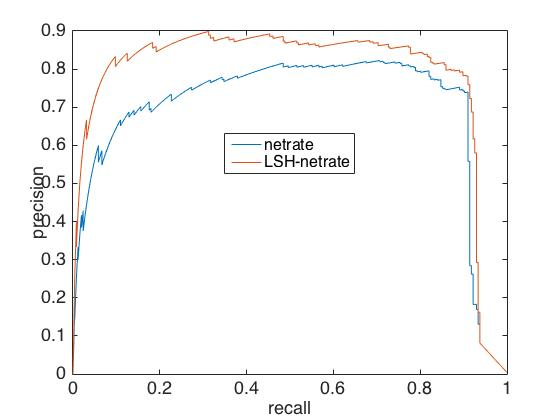
\includegraphics[width=0.35\linewidth]{figures/PR900.jpg}}
\subfigure[LSH-ConNie]{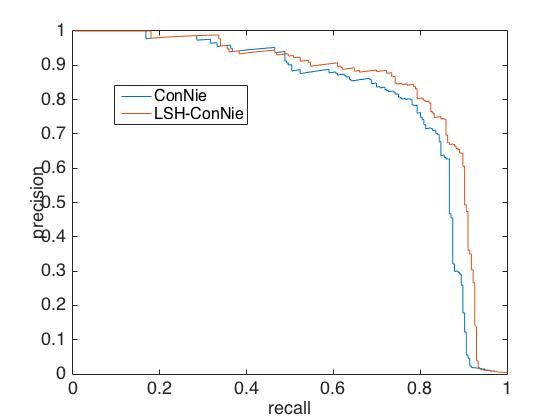
\includegraphics[width=0.35\linewidth]{figures/Connie900.jpg}}
\subfigure[LSH-NetInf]{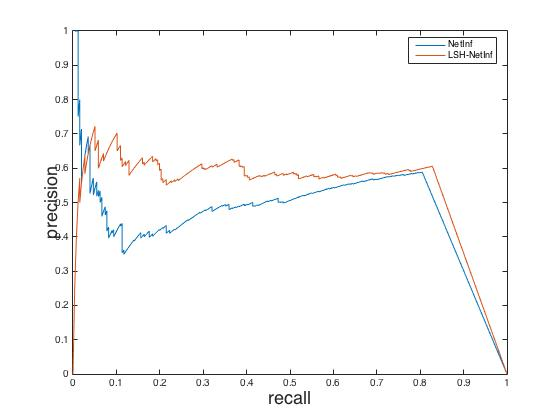
\includegraphics[width=0.35\linewidth]{figures/NetInfPR.jpg}}}
\caption{Precision-Recall curve of LSH-NetRate/LSH-ConNie/LSH-NetInf method }\label{fig:synLSHpr}
\end{figure*}
%--------------

\textbf{Performance vs. heterogeneity strength.} We generate synthetic cascades with various heterogeneity strength, as shown in Table \ref{tab:Spfunction}. The level of standard deviation depicts the strength of heterogeneity. Experiments in Figure \ref{fig:Hete} show that our method gains larger advantage to original NetRate as standard deviation of $P^c$ increases.
\begin{table}[H]
\caption{4 types of Sp function with different standard deviation.}
\begin{tabular}{c|c|c}
 & $P^c$ function & standard deviation \\
\hline
1 & [0.2 0.2 0.2 0.2 0.2] & 0\\
2 & [0.2 0.4 0.3 0.05 0.05] & 0.1541\\
3 & [0.1 0.6 0.3 0 0] & 0.2549\\
4 & [0.03 0.9 0.07 0 0] & 0.3924
\end{tabular}\label{tab:Spfunction}
\end{table}
\begin{figure}[H]
\centerline{
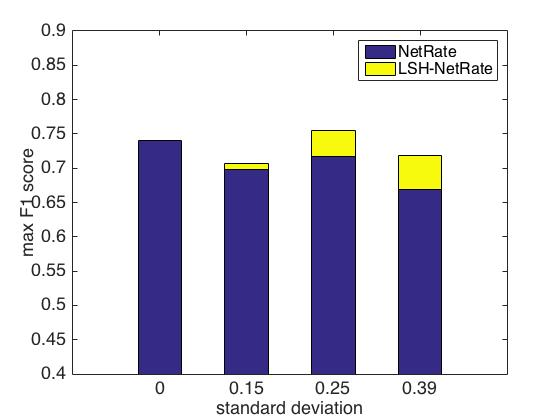
\includegraphics[width=0.75\linewidth]{figures/HeteroStrength.jpg}}
\caption{Experiments on different heterogeneity strength. }\label{fig:Hete}
\end{figure}
%--------------
\textbf{Setting of $L$.} $L$ is the length of sliding window around target time stamp that can affect the estimation of $P^c$. We run our methods with 4 different $L$ settings separately, results are shown in Figure \ref{fig:SetLAG}. We can see that their differences are slight as we change $L$'s value. But LSH method performs better with $L$ set around 10\% of T.
\begin{figure}[H]
\centerline{
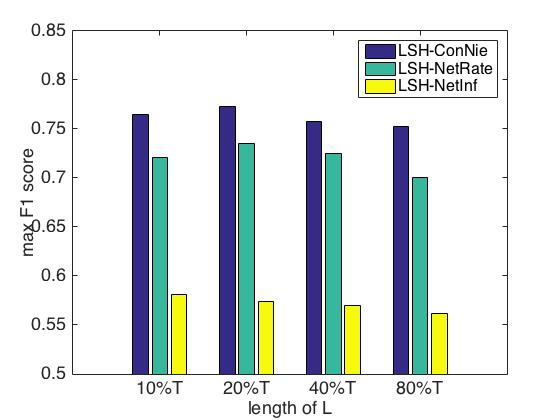
\includegraphics[width=0.75\linewidth]{figures/SettingLAG.jpg}}
\caption{Experiments of different $L$ values. }\label{fig:SetLAG}
\end{figure}
%--------------
\textbf{Experiments of CLSH method.}
CLSH method attempts to cluster cascades so that cascades in the same group have similar $P^c(t)$. In this part, we use 3 types of $P^c(t)$ functions: [0.1 0.8 0.1 0 0] / [0.8 0.2 0 0 0] / [0 0 0 0.2 0.8]. Before simulating each cascade, we randomly choose one of this three to be the specific $P^c$ function of this cascade.  

\textbf{Performance of CLSH vs. cascade number.} We make experiments of CLSH-NetRate/CLSH-ConNie/CLSH-NetInf methods on synthetic cascades with multiply heterogeneity functions. As shown in Table \ref{tab:synCLSHCASf1} and \ref{tab:synCLSHCASAUC}, our methods outperform the original algorithms on max $F_1$ score and $AUC$. 
\begin{table}[H]
\caption{Max $F_1$ score of CLSH-NetRate/CLSH-ConNie/CLSH-NetInf vs. casNum}
\begin{tabular}{c|c|c|c}
 & casNum 300 & casNum 600 & casNum 900 \\
\hline
NetRate & 0.7124 & 0.7222 & 0.7254\\
CLSH-NetRate & 0.7256 & 0.7425 & 0.7414\\
\hline
ConNie & 0.7296 & 0.7531 & 0.7619\\
CLSH-ConNie & 0.7474 & 0.7520 & 0.7692\\
\hline
NetInf & 0.6727 & 0.7133 & 0.7316\\
CLSH-NetInf & 0.6886 & 0.7314 & 0.7489
\end{tabular}\label{tab:synCLSHCASf1}
\end{table}
%---------------
\begin{table}[H]
\caption{Area under PR curve of CLSH-NetRate/CLSH-ConNie/CLSH-NetInf vs. casNum}
\begin{tabular}{c|c|c|c}
 & casNum 300 & casNum 600 & casNum 900 \\
\hline
NetRate & 0.5243 & 0.5445 & 0.5894\\
CLSH-NetRate & 0.5771 & 0.6527 & 0.6582\\
\hline
ConNie & 0.7006 & 0.7449 & 0.7612\\
CLSH-ConNie & 0.7194 & 0.7600 & 0.7602\\
\hline
NetInf & 0.4079 & 0.4248 & 0.5138\\
CLSH-NetInf & 0.4319 & 0.4402 & 0.5268
\end{tabular}\label{tab:synCLSHCASAUC}
\end{table}
\textbf{Setting of $k$.} As shown in Figure \ref{fig:SetK}, clustering cascades into 3 $\sim$ 4 groups produces higher accuracy.
\begin{figure}[H]
\centerline{
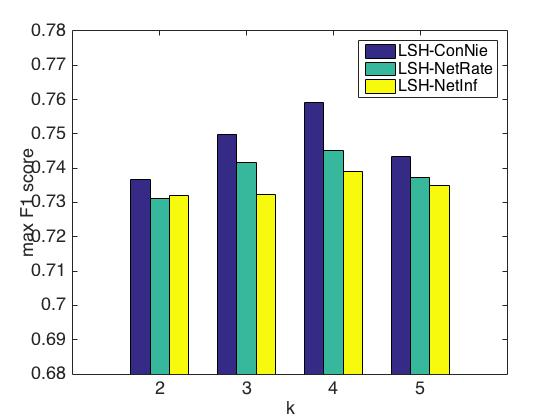
\includegraphics[width=0.75\linewidth]{figures/SettingK.jpg}}
\caption{Experiments of different k values. }\label{fig:SetK}
\end{figure}
%==========================
\subsection{Experiments on real world dataset}

\quad We use \emph{U.S. patent dataset} by \emph{the National Bureau of Economic Research} to test (C)LSH method. The dataset spans 25 years from 1975 to 1999, containing 16,522,438 citations. Inventors of patents cite their sources. Therefore, we take inventors as the entities of network and follow the citations to reveal information flow. Note that we remove all self-loops in patent data, which happen when inventors cite their own previous works. By ranking inventors according to their activity, we have 147 most active inventors to form the ground truth network. We extract 150/250/350/450 transmission trees for cascade information. Experiments of (C)LSH-NetRate, (C)LSH-ConNie, (C)LSH-NetInf are made on this dataset. 

For real world dataset, the lengths of cascades differ a lot. We apply Min-Max Normalization to activation times in each cascade separately. Cascades' length is 1 after transformation.
\begin{itemize}
\item (C)LSH-NetRate

\textbf{Performance vs. cascade number. }From Table \ref{tab:rwdLSHnetrateCASf1} we can see improvement by applying LSH method to NetRate on various data scale. Increasing $k$ in some occasions can help improve accuracy.
\begin{table}[H]
\caption{Real data: Max $F_1$ score of NetRate/  LSH-NetRate/ CLSH-NetRate vs. casNum}
\begin{tabular}{c|c|c|c|c}
 & cas 150 & cas 250 & cas 350 & cas 450 \\
 \hline
 NetRate & 0.5915 & 0.6110 & 0.6418 & 0.6667 \\
 LSH-NetRate & 0.6324 & 0.6364 & 0.6817 & 0.6975 \\
 CLSH-k 3 & 0.6328 & 0.6431 & 0.6731 & 0.6997 \\
 CLSH-k 5 & 0.6324 & 0.6360 & 0.6752 & 0.7121
\end{tabular}\label{tab:rwdLSHnetrateCASf1}
\end{table}
%--------------
\item (C)LSH-ConNie

\textbf{Performance vs. cascade number.} LSH method outperforms ConNie notably as shown in Table \ref{tab:rwdLSHconnieCASf1}. Furthermore, applying CLSH to cluster similar cascades extends the performance advantage over original ConNie method.
\begin{table}[H]
\caption{Real data: Max $F_1$ score of ConNie/  LSH-ConNie/ CLSH-ConNie vs. casNum}
\begin{tabular}{c|c|c|c|c}
 & cas 150 & cas 250 & cas 350 & cas 450 \\
 \hline
 ConNie & 0.5702 & 0.6127 & 0.6412 & 0.6788 \\
 LSH-ConNie & 0.8125 & 0.8222 & 0.8532 & 0.8673 \\
 CLSH-k 3 & 0.8249 & 0.8298 & 0.8502 & 0.8733 \\
 CLSH-k 5 & 0.8140 & 0.8218 & 0.8561 & 0.8581
\end{tabular}\label{tab:rwdLSHconnieCASf1}
\end{table}
%--------------
\item (C)LSH-NetInf

\textbf{Performance vs. cascade number.} Table \ref{tab:rwdLSHnetinfCASf1} and \ref{tab:rwdLSHnetinfCASauc} present the AUC and maximum $F_1$ score results of our methods and NetInf algorithm. In all cases, our methods perform better than NetInf. When including more cascades, the complexity increases. Proper increment of $k$ may lead to higher performance.
\begin{table}[H]
\caption{Real data: Max $F_1$ score of NetInf/  LSH-NetInf/ CLSH-NetInf vs. casNum}
\begin{tabular}{c|c|c|c|c}
 & cas 150 & cas 250 & cas 350 & cas 450 \\
 \hline
 NetInf & 0.5284 & 0.5382 & 0.5779 & 0.5981 \\
 LSH-NetInf & 0.7604 & 0.7762 & 0.7993 & 0.7932 \\
 CLSH-k 3 & 0.7757 & 0.7902 & 0.8000 & 0.7938 \\
 CLSH-k 5 & 0.7833 & 0.7762 & 0.8129 & 0.8062
\end{tabular}\label{tab:rwdLSHnetinfCASf1}
\end{table}
\begin{table}[H]
\caption{Real data: AUC of NetInf/ LSH-NetInf/ CLSH-NetInf vs. casNum}
\begin{tabular}{c|c|c|c|c}
 & cas 150 & cas 250 & cas 350 & cas 450 \\
 \hline
 NetInf & 0.7860 & 0.7919 & 0.8160 & 0.8292 \\
 LSH-NetInf & 0.9413 & 0.9393 & 0.9410 & 0.9429 \\
 CLSH-k 3 & 0.9502 & 0.9473 & 0.9418 & 0.9436 \\
 CLSH-k 5 & 0.9547 & 0.9393 & 0.9490 & 0.9506
\end{tabular}\label{tab:rwdLSHnetinfCASauc}
\end{table}
\end{itemize}
%&&&&&&&&&&&&&&&&&&&&&&&&&&&&&&&&&&
\section{Conclusions}
In this article, we design $Life~ Stage~Heuristics$ method, called $LSH$, to improve the accuracy of Network Inference by making use of heterogeneous influence strength information. In contrast to previous Network Inference algorithms, such as NetRate, ConNie and NetInf, our method considers the fact that the popularity of a story(patent product, etc) changes with time and we propose an efficient approach to learn the popularity heterogeneous networks. Experiments on both synthetic dataset and real world dataset show that our method outperforms the original NetRate, ConNie, and NetInf models. 
%&&&&&&&&&&&&&&&&&&&&&&&&&&&&&&&&&&
\bibliographystyle{aaai}
\bibliography{misc,names,conferences,theory_submodular,theory_InfMax,ml_NetworkInference,ml_TopicModel,ml_NetworkModel,optimization}

\end{document}
